\section{Bayesian Quadrature}
A major issue with the Riemannian LA is the computational cost of solving the IVP-problem. In the following, we will discuss how to remedy this by using Bayesian quadrature to efficiently find the integral in equation \ref{eq:posterior_predictive}.

Bayesian quadrature is a numerical method for integrating a function $f(\theta)$ over some measure $\pi(\theta)$: $J = \int f(\theta)\pi(\theta)d\theta$.
Briefly speaking, the assumption is that the function we want to integrate is drawn from a Gaussian Process distribution. Then the integral $J$ is a random variable and given a set of observations of $\theta$ and $f(\theta)$, the mean and variance of $J$ can be found. If the integration measure $\pi$ furthermore is Gaussian, the mean and variance has an analytical solution \cite{Bayesian_quadrature}. 

The amount of expected variance reduction gain from a new datapoint is measured by the acquisition function, and by maximizing this function it is computationally feasible to find the next value of $\theta$ that will minimize the variance of $J$. Figure \ref{fig:UFA_BQ_integrand_vals_1d} shows then mean and variance of a Gaussian Process conditioned on three data points as an illustration. The corresponding function values and variance multiplied by the integration measure is seen in figure \ref{fig:UFA_BQ_integrand_vals_measure_1d}.

\begin{figure}[h]
    \centering
    \subfloat[Integrand values]{
        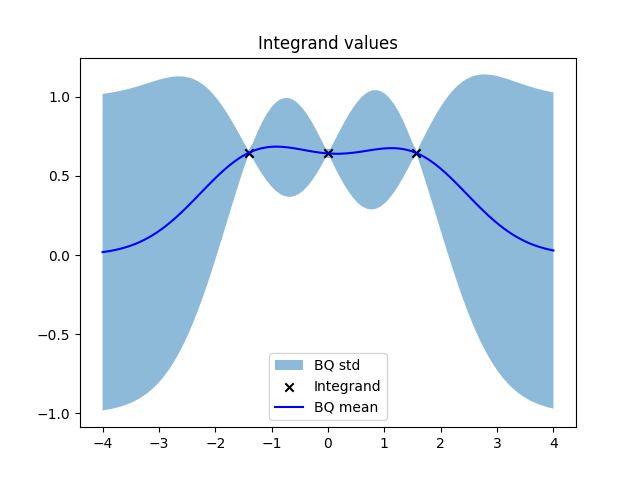
\includegraphics[width=.31\linewidth]{report/figures/UFA_BQ_integrand_vals_1d.png}
        \label{fig:UFA_BQ_integrand_vals_1d}
    }
    \hfill
    \subfloat[Integrand values and measure]{
        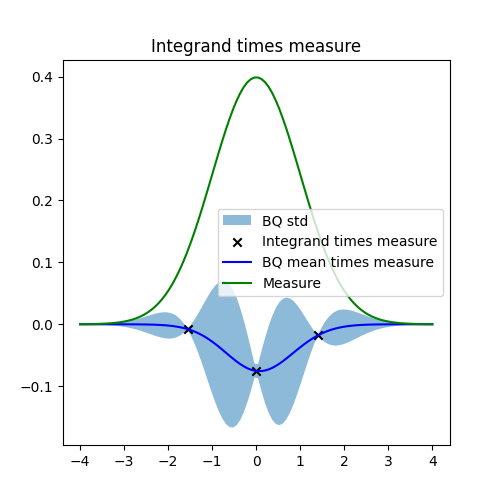
\includegraphics[width=.31\linewidth]{report/figures/UFA_BQ_integrand_vals_measure_1d.png}
        \label{fig:UFA_BQ_integrand_vals_measure_1d}
    }
    \hfill
    \caption{Bayesian Quadrature approximation}
    \label{fig:bayesian_quadrature1}
\end{figure}


In our case, $f(\theta)=p(t^\ast\vert x^\ast, \theta)$ and $\pi(\theta) = p(\theta\vert \mathcal{D})$. 
As discussed in the previous section we approximate $p(\theta\vert \mathcal{D})$ by the Riemannian LA denoted by $q_\theta(\theta)$ where $\theta=\text{Exp}_{\theta^\ast}(v)$ and $v\sim \mathcal N(\theta^\ast, \Sigma_{\theta^\ast})$. Then $v=\text{Log}_{\theta^\ast}(\theta)$ and if the distribution of $v$ is given as $q_v(v)$, following \cite[p.29]{tomczak2024deep} we get that

\begin{align}
q_\theta(\theta) &= q_v(\text{Log}_{\theta^\ast}(\theta)) \cdot \left\vert \det\left( \left. \frac{\partial \text{Log}_{\theta^\ast}(z)}{\partial z}\right\vert_{z=\theta}\right) \right\vert \\
&= q_v(\text{Log}_{\theta^\ast}(\theta)) \cdot \left\vert \det\left( \left. \frac{\partial \text{Exp}_{\theta^\ast}(z)}{\partial z}\right\vert_{z=\text{Log}_{\theta^\ast}(\theta)}\right) \right\vert^{-1} \\
&= q_v(\text{Log}_{\theta^\ast}(\theta)) \cdot \left\vert J[{\text{Exp}_{\theta^\ast}}](\text{Log}_{\theta^\ast}(\theta)) \right\vert^{-1} \\
\end{align}
from which we can conclude that 
\begin{align*}
    q_v(v) = q_\theta(\text{Exp}_{\theta^\ast}(v)) \cdot \left\vert J[{\text{Exp}_{\theta^\ast}}](v) \right\vert
\end{align*}
We can expand on the primary integral with integration by substitution and get
\begin{align*}
J 
&= \int f(\theta) q(\theta)d\theta \\
&= \int f(\text{Exp}_{\theta^\ast}(v)) \cdot q_\theta(\text{Exp}_{\theta^\ast}(v)) \cdot \vert J[{\text{Exp}_{\theta^\ast}}](v) \vert dv \\
&= \int f(\text{Exp}_{\theta^\ast}(v)) \cdot q_v(v) dv
\end{align*}
Since $q_v(v)$ is Gaussian, we can use this as measure for the Bayesian quadrature, and then integrate the function $f(\text{Exp}_{\theta^\ast}(v))$.

In figure \ref{fig:UFA_BQ_variance}, the Bayesian Quadrature Riemannian Laplace approximation (BQ-Riemann) for the function approximator is plotted with the corresponding 95\% band for the mean and for the observations. 

\begin{figure}[h]
    \centering
        \subfloat[Riemannian Laplace approximation for the function approximator]{
        \label{fig:UFA_riemannian_subspace_rank1}
        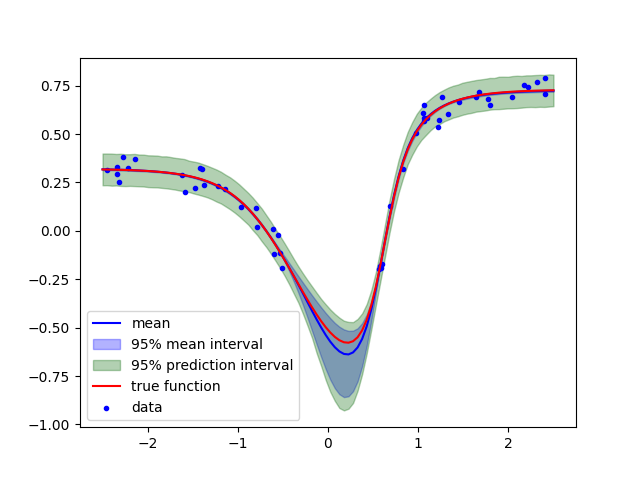
\includegraphics[width=.45\linewidth]{report/figures/UFA_riemannian_subspace_rank2.png}
    }
    \hfill
    \subfloat[Bayesian Quadrature Riemannian Laplace approximation for the function approximator]{
        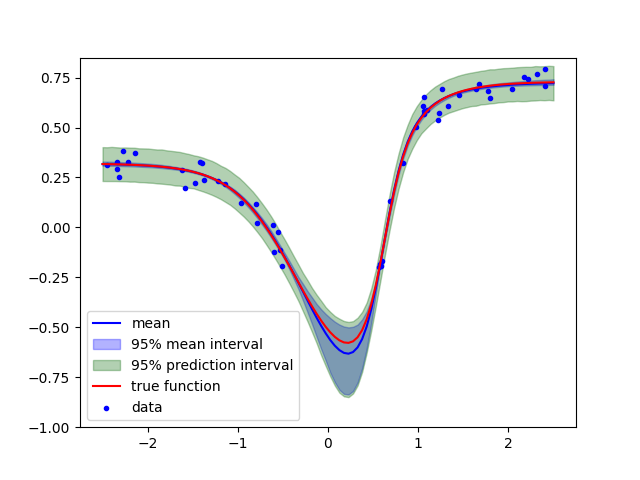
\includegraphics[width=.45\linewidth]{report/figures/UFA_riemannian_BQ_subspace_rank2.png}
        \label{fig:UFA_BQ_variance}
    }
    \caption{Function approximator}

    \label{fig:bayesian_quadrature2}
\end{figure}

